\documentclass[utf8,compress]{beamer}
\usepackage{irbookslide}
\usepackage{irilmenau2}
\usepackage{url}
\usepackage{fontspec} % zahteva paket euenc
\usepackage{xunicode}
\usepackage{xltxtra}
\usepackage{polyglossia}
\usepackage{minted}
\usepackage{xcolor,colortbl}
\usepackage{textcomp}
\usepackage{unicode-math}

\title{GUI aplikacije i PyQt}
\subtitle{\tiny{Slajdovi za predmet Osnove programiranja}}
\subject{Osnove programiranja}
\institute{Katedra za informatiku, Fakultet tehničkih nauka, Novi Sad}
\date{2014.}

\begin{document}
% da pygmentize ne uokviruje crvenom bojom nepoznate karaktere
\expandafter\def\csname PY@tok@err\endcsname{}

\frame{\titlepage}

\frame{
  \frametitle{Ciljevi}
  \begin{itemize}
    \item GUI = graphical user interface
    \item savlađivanje osnovnih koncepata pisanja GUI aplikacija
  \end{itemize}
}

\section[PyQt]{PyQt}

\begin{frame}[fragile]
  \frametitle{GUI biblioteke i Python}
  \begin{itemize}
    \item pisanje programa koji ima GUI od nule je ogroman posao
    \item puno istih funkcija bismo morali da pišemo iznova za svaki program
    \item $\Rightarrow$ možemo da koristimo \myblue{biblioteku klasa}
    \item za Python ih ima mnogo:
    \begin{itemize}
      \item TkInter
      \item wxPython
      \item PyQt
      \item PyGTK
      \item ...
    \end{itemize}
  \end{itemize}
\end{frame}

\begin{frame}[fragile]
  \frametitle{PyQt}
  \begin{itemize}
    \item Qt je cross-platform biblioteka za C++
    \begin{itemize}
      \item Windows, Linux, Mac OSX, Symbian, Android, iOS
    \end{itemize}
    \item PyQt je Python omotač oko Qt biblioteke
  \end{itemize}
\end{frame}

\begin{frame}[fragile]
  \frametitle{Struktura GUI aplikacije}
  \begin{itemize}
    \item bez obzira na izabranu GUI biblioteku, svaki program ima sličnu strukturu
    \item program se ne izvršava linearno (od početka prema kraju, bez pauze), već se izvršava samo u pojedinim trenucima \\ \ \\
    \item[1] inicijalizacija programa prilikom pokretanja 
    \begin{itemize}
      \item inicijalizuju se interne strukture podataka
    \end{itemize}
    \item[2] prepuštanje kontrole OS-u i čekanje na događaje
    \begin{itemize}
      \item mouse click, key press, touch, swipe, ...
    \end{itemize}
    \item[3] obrada nastalog događaja i prelazak na \myblue{2}
  \end{itemize}
\end{frame}

\begin{frame}[fragile]
  \frametitle{Prva GUI aplikacija}
\begin{minted}{python}
import sys
from PyQt4 import QtGui

def main():
    # inicijalizacija
    app = QtGui.QApplication(sys.argv)
    w = QtGui.QWidget()
    w.resize(250, 150)
    w.move(300, 300)
    w.setWindowTitle('Prvi GUI program')
    w.show()
    # ovde je petlja za obradu događaja
    sys.exit(app.exec_())

if __name__ == '__main__':
    main()
\end{minted}
\end{frame}

\begin{frame}[fragile]
  \frametitle{Struktura GUI aplikacije}
  \begin{itemize}
    \item prozor već ima dosta funkcionalnosti (close, resize)
    \item nismo morali da pišemo sve od početka
  \end{itemize}
  \begin{center}
    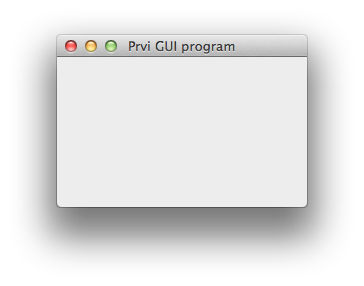
\includegraphics[width=8cm]{pyqt01.png}
  \end{center}
\end{frame}

\section[Bars]{Status bar, menu bar, toolbar}

\begin{frame}[fragile]
  \frametitle{Dodajemo status bar}
\begin{minted}{python}
class Example(QtGui.QMainWindow):
    def __init__(self):
        super(Example, self).__init__()
        self.initUI()
        
    def initUI(self):               
        # ovde se uključuje status bar
        self.statusBar().showMessage('Ready')
        self.setGeometry(300, 300, 250, 150)
        self.setWindowTitle('Statusbar')    
        self.show()

def main():    
    app = QtGui.QApplication(sys.argv)
    ex = Example()
    sys.exit(app.exec_())
\end{minted}
\end{frame}

\begin{frame}[fragile]
  \frametitle{Dodajemo status bar $_2$}
  \begin{itemize}
    \item tekst u status baru se definiše pomoću \texttt{setMessage}
  \end{itemize}
  \begin{center}
    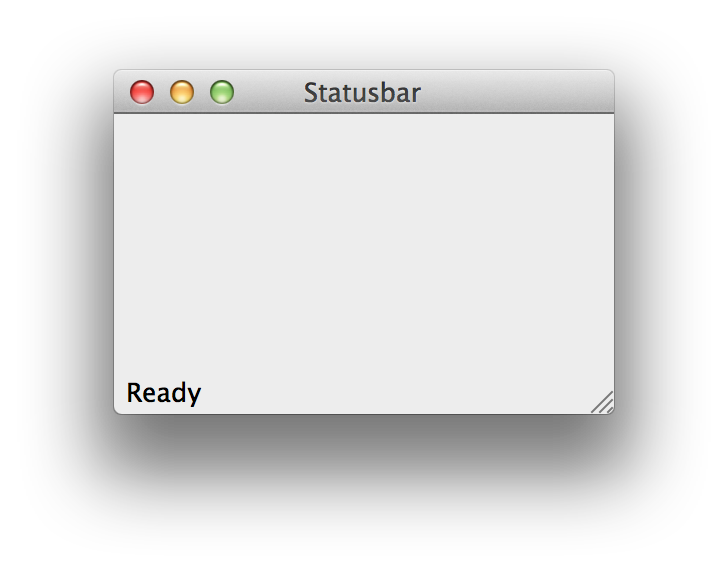
\includegraphics[width=8cm]{pyqt02.png}
  \end{center}
\end{frame}


\begin{frame}[fragile]
  \frametitle{Dodajemo meni}
\begin{minted}{python}
class Example(QtGui.QMainWindow):
    def initUI(self):                       
        exitAction = QtGui.QAction(QtGui.QIcon('exit.png'), '&Exit', self)        
        exitAction.setShortcut('Ctrl+Q')
        exitAction.setStatusTip('Exit application')
        exitAction.triggered.connect(QtGui.qApp.quit)

        self.statusBar().showMessage('Ready')
        menubar = self.menuBar()
        fileMenu = menubar.addMenu('&File')
        fileMenu.addAction(exitAction)
        
        self.setGeometry(300, 300, 300, 200)
        self.setWindowTitle('Menubar')    
        self.show()
\end{minted}
\end{frame}

\begin{frame}[fragile]
  \frametitle{Dodajemo meni $_2$}
  \begin{itemize}
    \item klik na stavku menija ili Ctrl-Q ili Alt-F,E zatvaraju program
  \end{itemize}
  \begin{center}
    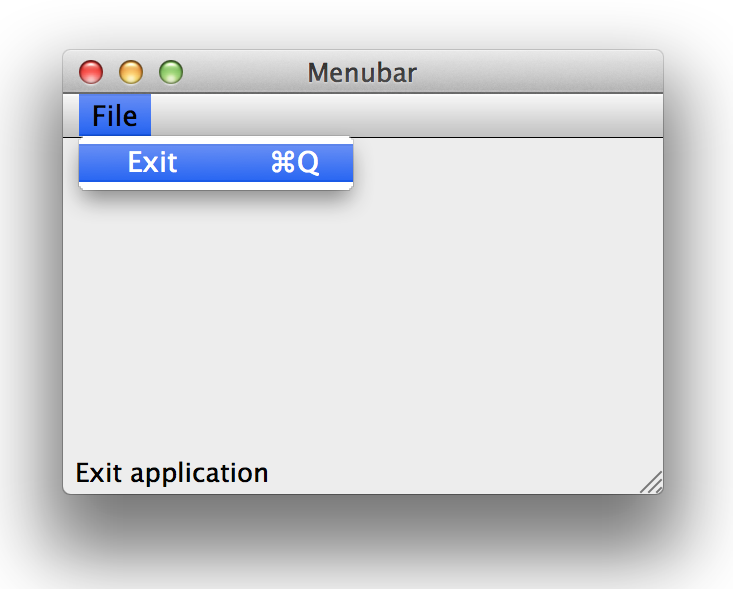
\includegraphics[width=8cm]{pyqt03.png}
  \end{center}
\end{frame}

\begin{frame}[fragile]
  \frametitle{Dodajemo toolbar}
\begin{minted}{python}
class Example(QtGui.QMainWindow):
    def initUI(self):
        ...
        self.toolbar = self.addToolBar('Exit')
        self.toolbar.addAction(exitAction)        
\end{minted}
\begin{center}
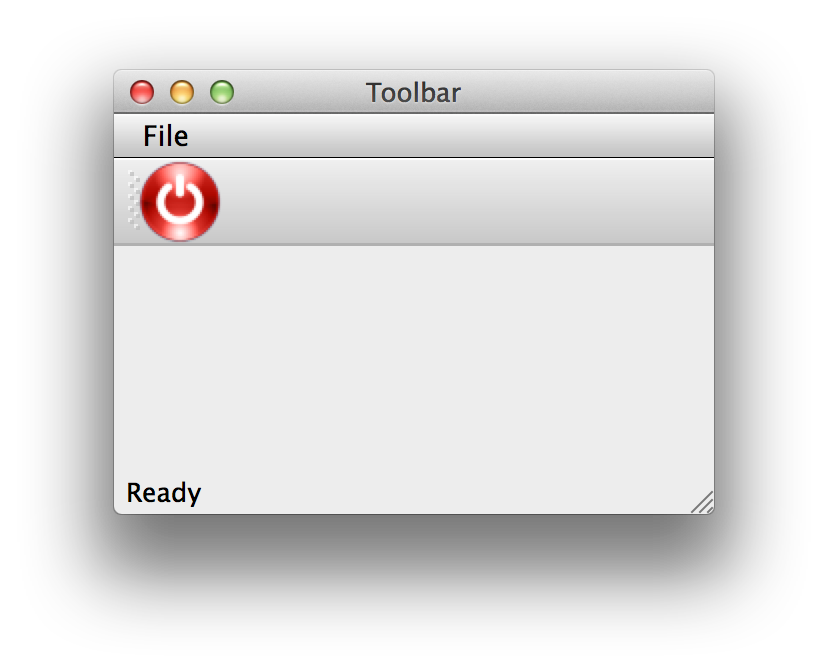
\includegraphics[width=8cm]{pyqt04.png}
\end{center}
\end{frame}

\section[Pozicioniranje]{Pozicioniranje komponenti u prozoru}

\begin{frame}[fragile]
  \frametitle{Raspored komponenti na prozoru}
  \begin{itemize}
    \item komponente (widgets) se mogu rasporediti na više načina
    \item[1] apsolutno pozicioniranje (piksel koordinate)
    \item[2] neki drugi način
  \end{itemize}
\end{frame}

\begin{frame}[fragile]
  \frametitle{Apsolutno pozicioniranje}
\begin{minted}{python}
class Example(QtGui.QMainWindow):
    def initUI(self):
        ...
        lbl1 = QtGui.QLabel('Apsolutno', self)
        lbl1.move(15, 10)
        lbl2 = QtGui.QLabel('pozicioniranje', self)
        lbl2.move(35, 40)
        lbl3 = QtGui.QLabel('komponenti', self)
        lbl3.move(55, 70)        
        self.show()
\end{minted}
\end{frame}

\begin{frame}[fragile,shrink]
  \frametitle{Apsolutno pozicioniranje $_2$}
\begin{center}
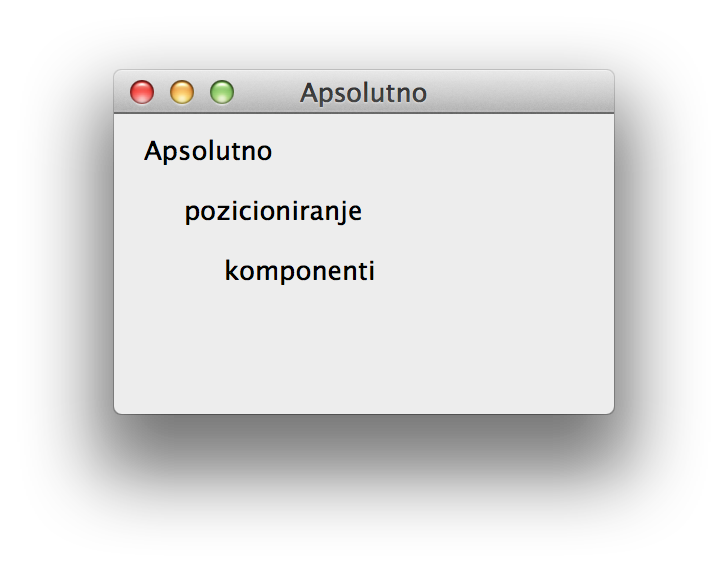
\includegraphics[width=8cm]{pyqt05.png}
\end{center}
  \begin{itemize}
    \item teško je prilagoditi prikaz različitim uslovima
    \begin{itemize}
      \item različiti OS
      \item različita veličina osnovnog fonta
    \end{itemize}
  \end{itemize}
\end{frame}

\begin{frame}[fragile]
  \frametitle{Pozicioniranje komponenti: Box Layout}
\begin{minted}{python}
class Example(QtGui.QMainWindow):
    def initUI(self):
        ...
        okButton = QtGui.QPushButton("OK")
        cancelButton = QtGui.QPushButton("Cancel")
        hbox = QtGui.QHBoxLayout()
        hbox.addStretch(1)
        hbox.addWidget(okButton)
        hbox.addWidget(cancelButton)
        vbox = QtGui.QVBoxLayout()
        vbox.addStretch(1)
        vbox.addLayout(hbox)
        self.setLayout(vbox)    
\end{minted}
\end{frame}

\begin{frame}[fragile]
  \frametitle{Pozicioniranje komponenti: Box Layout $_2$}
\begin{center}
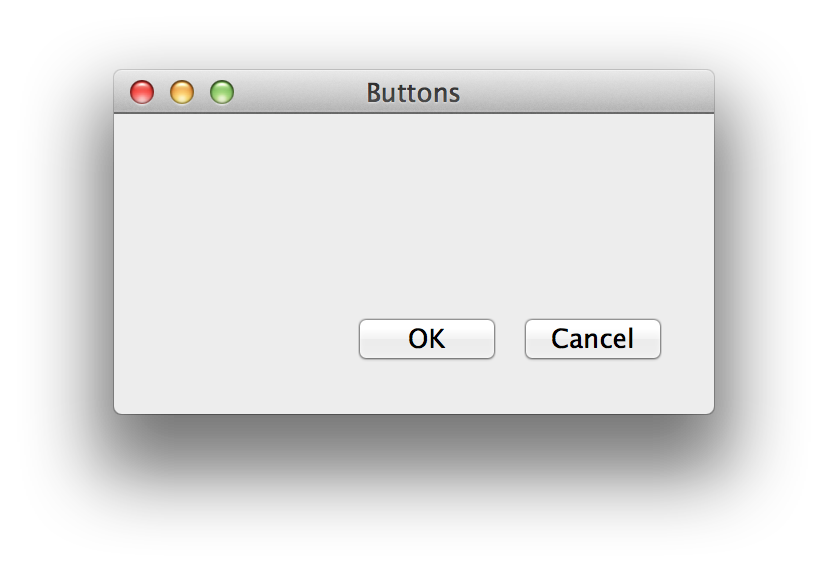
\includegraphics[scale=0.4]{pyqt06.png}
\end{center}
  \begin{itemize}
    \item OK i Cancel su u horizontalnom boxu, gurnuti u desno
    \item horizontalni box je u vertikalnom boxu, gurnut na dole
  \end{itemize}
\end{frame}

\begin{frame}[fragile]
  \frametitle{Pozicioniranje komponenti: Box Layout $_3$}
\begin{center}
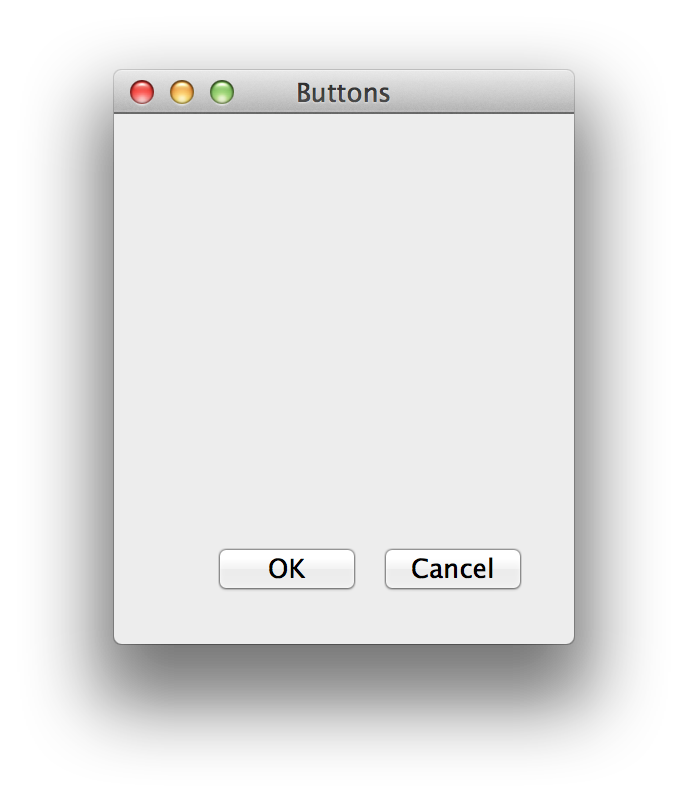
\includegraphics[scale=0.4]{pyqt07.png}
\end{center}
  \begin{itemize}
    \item isti odnos je i nakon promene veličine prozora
  \end{itemize}
\end{frame}

\begin{frame}[fragile,shrink=8]
  \frametitle{Pozicioniranje komponenti: QGridLayout}
\begin{minted}{python}
class Example(QtGui.QMainWindow):
    def initUI(self):
        ...
        grid = QtGui.QGridLayout()
        self.setLayout(grid)
        names = ['Cls', 'Bck', '', 'Close',
                 '7', '8', '9', '/',
                 '4', '5', '6', '*',
                 '1', '2', '3', '-',
                 '0', '.', '=', '+']
        positions = [(i,j) for i in range(5) for j in range(4)]
        for position, name in zip(positions, names):
            if name == '':
                continue
            button = QtGui.QPushButton(name)
            grid.addWidget(button, *position)
\end{minted}
\end{frame}

\begin{frame}[fragile]
  \frametitle{Pozicioniranje komponenti: QGridLayout $_2$}
\begin{center}
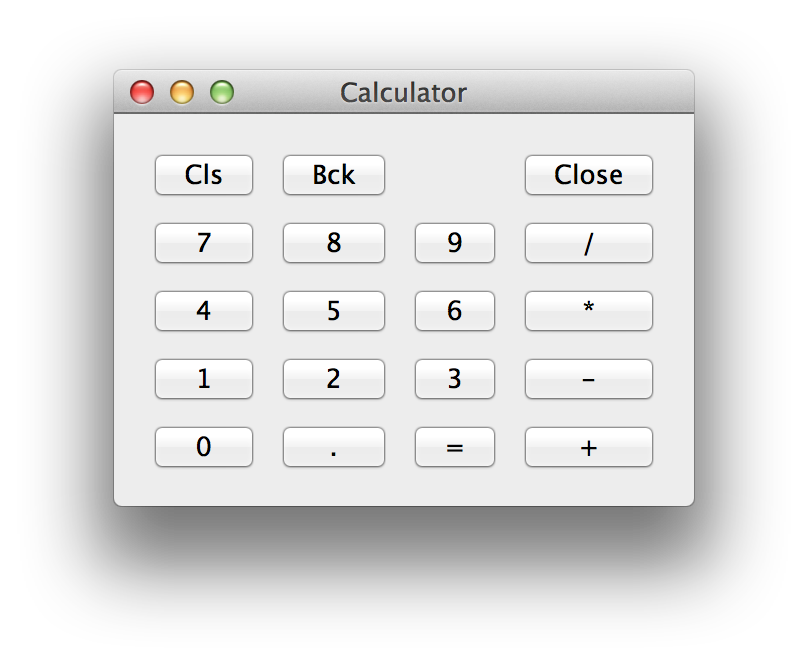
\includegraphics[scale=0.5]{pyqt08.png}
\end{center}
  \begin{itemize}
    \item raspored je otporan na promenu veličine prozora
  \end{itemize}
\end{frame}

\begin{frame}[fragile,shrink=20]
  \frametitle{Pozicioniranje komponenti: QGridLayout $_3$}
  \begin{itemize}
    \item komponente mogu da se prostiru preko više kolona ili redova
  \end{itemize}
\begin{minted}{python}
class Example(QtGui.QMainWindow):
    def initUI(self):
        ...
        title = QtGui.QLabel('Title'); author = QtGui.QLabel('Author')
        review = QtGui.QLabel('Review'); titleEdit = QtGui.QLineEdit()
        authorEdit = QtGui.QLineEdit(); reviewEdit = QtGui.QTextEdit()
        grid = QtGui.QGridLayout()
        grid.setSpacing(10)
        grid.addWidget(title, 1, 0)
        grid.addWidget(titleEdit, 1, 1)
        grid.addWidget(author, 2, 0)
        grid.addWidget(authorEdit, 2, 1)
        grid.addWidget(review, 3, 0)
        # reviewEdit se prostire preko 5 redova
        grid.addWidget(reviewEdit, 3, 1, 5, 1)
        self.setLayout(grid)
\end{minted}
\end{frame}

\begin{frame}[fragile]
  \frametitle{Pozicioniranje komponenti: QGridLayout $_4$}
\begin{center}
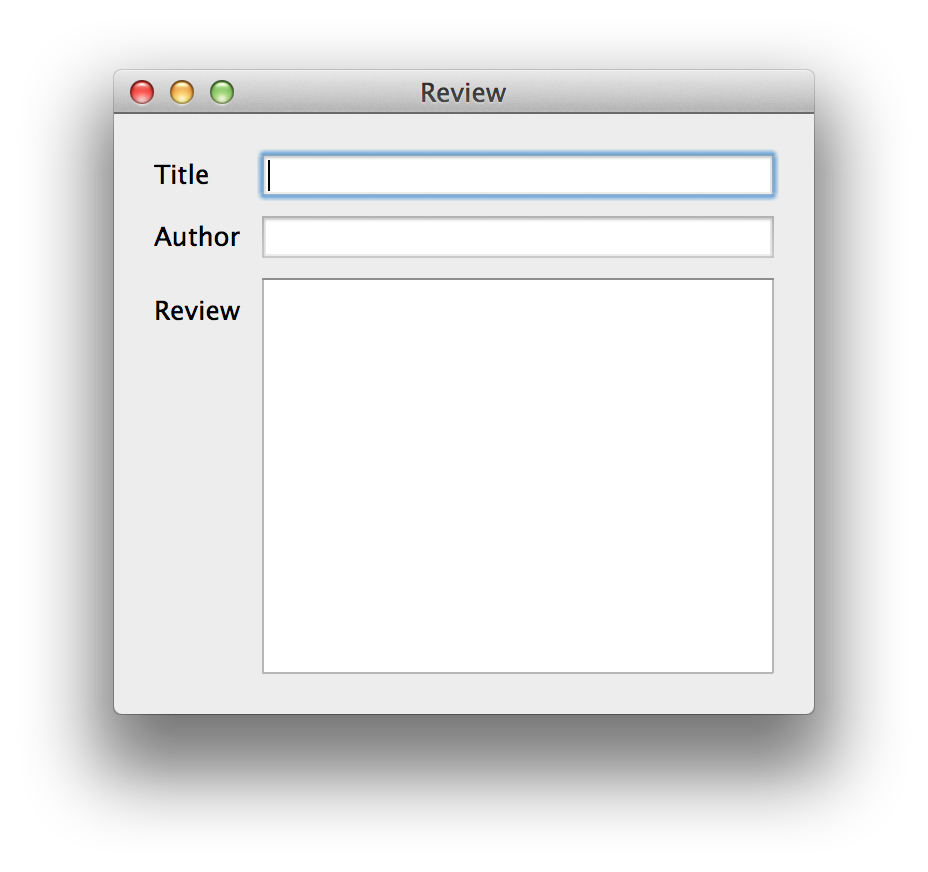
\includegraphics[scale=0.5]{pyqt09.png}
\end{center}
\end{frame}

\section[Slots+Signals]{Događaji i signali}

\begin{frame}[fragile]
  \frametitle{Događaji u korisničkom interfejsu}
  \begin{itemize}
    \item za svaki događaj vezane su tri stvari
    \begin{itemize}
      \item izvor: objekat čije stanje se menja
      \item objekat: enkapsulira promenu stanja
      \item odredište: želi da bude obavešten o događaju
    \end{itemize}
    \item \myblue{signal} se emituje kada se desi događaj
    \item \myblue{slot} se poziva kada se desi događaj
  \end{itemize}
\begin{minted}{python}
button.clicked.connect(self.onClick)
\end{minted}
  \begin{itemize}
    \item izvor: \texttt{button}
    \item signal: \texttt{clicked}
    \item slot: \texttt{onClick()}
  \end{itemize}
\end{frame}

\begin{frame}[fragile,shrink]
  \frametitle{Signal/slot primer}
\begin{minted}{python}
class Example(QtGui.QWidget):
    def initUI(self):
        ...
        lcd = QtGui.QLCDNumber(self)
        sld = QtGui.QSlider(QtCore.Qt.Horizontal, self)
        vbox = QtGui.QVBoxLayout()
        vbox.addWidget(lcd)
        vbox.addWidget(sld)
        self.setLayout(vbox)
        # source: sld
        # signal: valueChanged
        # slot: lcd.display
        sld.valueChanged.connect(lcd.display)
\end{minted}
\end{frame}

\begin{frame}[fragile]
  \frametitle{Signal/slot primer $_2$}
\begin{center}
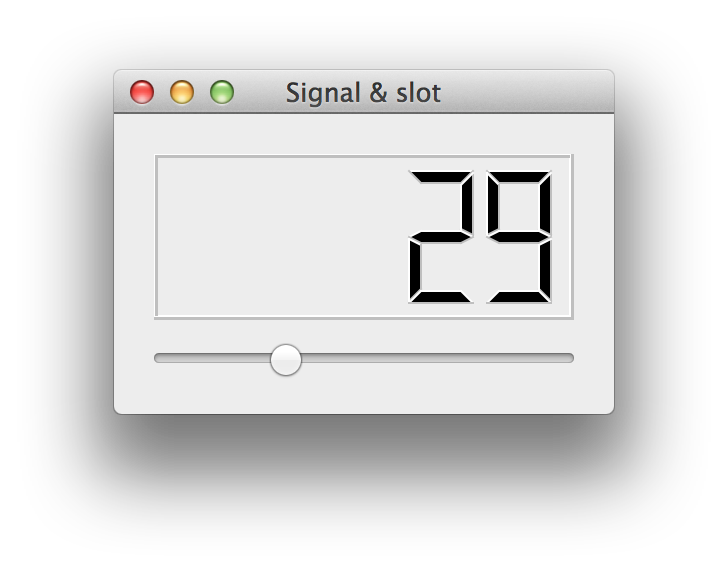
\includegraphics[scale=0.5]{pyqt10.png}
\end{center}
\end{frame}

\begin{frame}[fragile]
  \frametitle{Redefinisanje postojeće obrade događaja}
\begin{minted}{python}
class Example(QtGui.QWidget):
    # nasleđena metoda, poziva se na pritisak tastera
    # redefinišemo je u našem nasledniku QWidget-a
    def keyPressEvent(self, e):
        if e.key() == QtCore.Qt.Key_Escape:
            self.close() 
\end{minted}
\end{frame}

\begin{frame}[fragile]
  \frametitle{Informacije o izvoru događaja}
\begin{minted}{python}
class Example(QtGui.QMainWindow):
    def initUI(self):      
        btn1 = QtGui.QPushButton("Button 1", self)
        btn1.move(30, 50)
        btn2 = QtGui.QPushButton("Button 2", self)
        btn2.move(150, 50)
        btn1.clicked.connect(self.buttonClicked)            
        btn2.clicked.connect(self.buttonClicked)
        self.statusBar()
        ...
    def buttonClicked(self):
        # zbog koga sam pozvan?      
        sender = self.sender()
        self.statusBar().showMessage(sender.text() + 
            ' was pressed')
\end{minted}
\end{frame}

\begin{frame}[fragile]
  \frametitle{Informacije o izvoru događaja $_2$}
\begin{center}
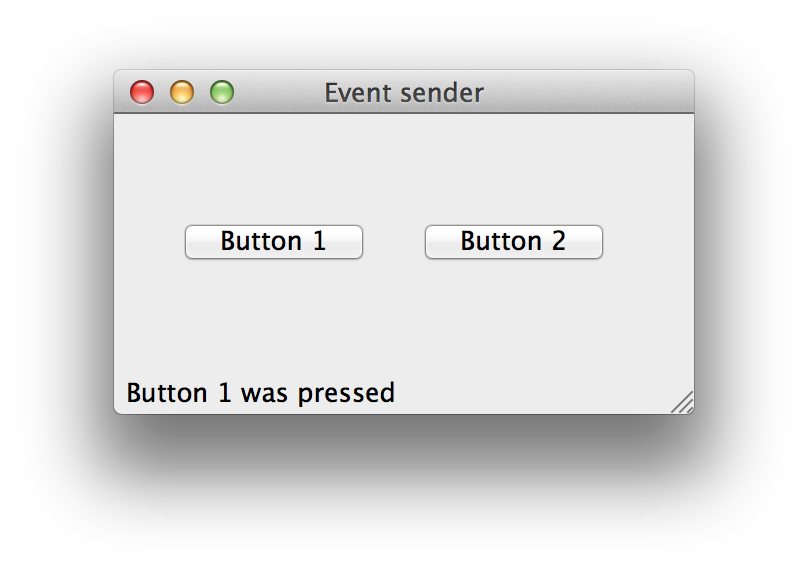
\includegraphics[scale=0.5]{pyqt11.png}
\end{center}
\end{frame}

\begin{frame}[fragile]
  \frametitle{Definisanje nove vrste događaja}
\begin{minted}{python}
class Example(QtGui.QMainWindow):
    # closeApp je novi signal
    closeApp = QtCore.pyqtSignal() 

    def initUI(self):
        # poveži closeApp sa close() slotom
        # close zatvara aplikaciju
        self.closeApp.connect(self.close)
        ...
        
    def mousePressEvent(self, event):
        # emituj događaj kad se klikne mišem
        self.closeApp.emit()
\end{minted}
\end{frame}

\section[Widgets]{Komponente interfejsa}

\begin{frame}[fragile]
  \frametitle{QCheckBox}
\begin{minted}{python}
class Example(QtGui.QMainWindow):
    def initUI(self):
        cb = QtGui.QCheckBox('Prikazi naslov', self)
        cb.move(20, 20)
        cb.toggle()
        cb.stateChanged.connect(self.changeTitle)
        ...
        
    def changeTitle(self, state):      
        if state == QtCore.Qt.Checked:
            self.setWindowTitle('Naslov')
        else:
            self.setWindowTitle('')
\end{minted}
\end{frame}

\begin{frame}[fragile]
  \frametitle{QCheckBox $_2$}
\begin{center}
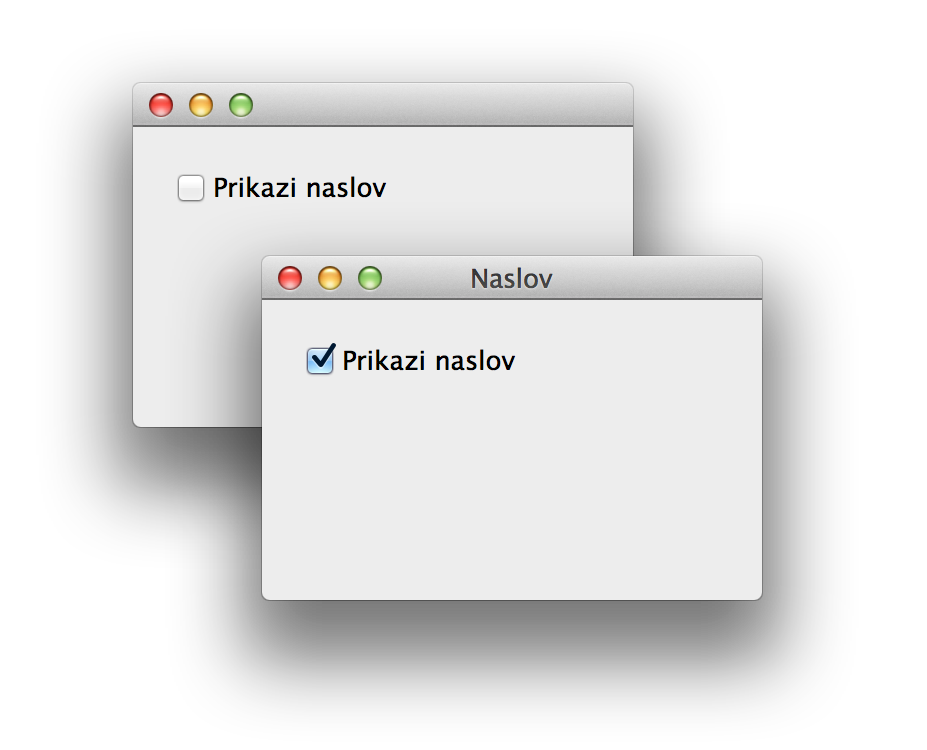
\includegraphics[scale=0.25]{pyqt12.png}
\end{center}
\end{frame}

\begin{frame}[fragile,shrink]
  \frametitle{QPushButton}
\begin{minted}{python}
class Example(QtGui.QMainWindow):
    def initUI(self):
        redb = QtGui.QPushButton('Red', self)
        redb.setCheckable(True)  # dugme sa dva stanja!
        redb.move(10, 10)
        # signal prenosi bool parametar!
        redb.clicked[bool].connect(self.setColor)
        ...
        self.square = QtGui.QFrame(self)
        self.square.setGeometry(150, 20, 100, 100)
        ...
    def setColor(self, pressed):
        source = self.sender()
        if pressed:
            ...
\end{minted}
\end{frame}

\begin{frame}[fragile]
  \frametitle{QPushButton $_2$}
\begin{center}
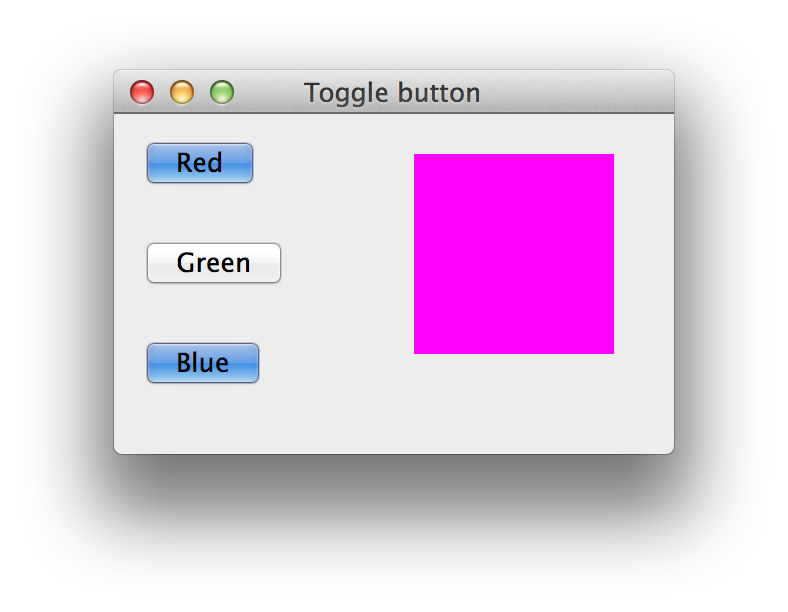
\includegraphics[scale=0.5]{pyqt13.png}
\end{center}
\end{frame}

\begin{frame}[fragile,shrink]
  \frametitle{QSlider}
\begin{minted}{python}
class Example(QtGui.QMainWindow):
    def initUI(self):
        sld = QtGui.QSlider(QtCore.Qt.Horizontal, self)
        sld.setFocusPolicy(QtCore.Qt.NoFocus)
        sld.setGeometry(30, 40, 100, 30)
        # signal prenosi int parametar!
        sld.valueChanged[int].connect(self.changeValue)
        ...
        self.label = QtGui.QLabel(self)
        self.label.setPixmap(QtGui.QPixmap('mute.png'))
        self.label.setGeometry(160, 40, 80, 30)
        ...
    def changeValue(self, value):
        if value == 0:
            self.label.setPixmap(QtGui.QPixmap('mute.png'))
        elif value > 0 and value <= 30:
            self.label.setPixmap(QtGui.QPixmap('min.png'))
        elif value > 30 and value < 80:
            self.label.setPixmap(QtGui.QPixmap('mid.png'))
        else:
            self.label.setPixmap(QtGui.QPixmap('max.png'))
\end{minted}
\end{frame}

\begin{frame}[fragile]
  \frametitle{QSlider $_2$}
\begin{center}
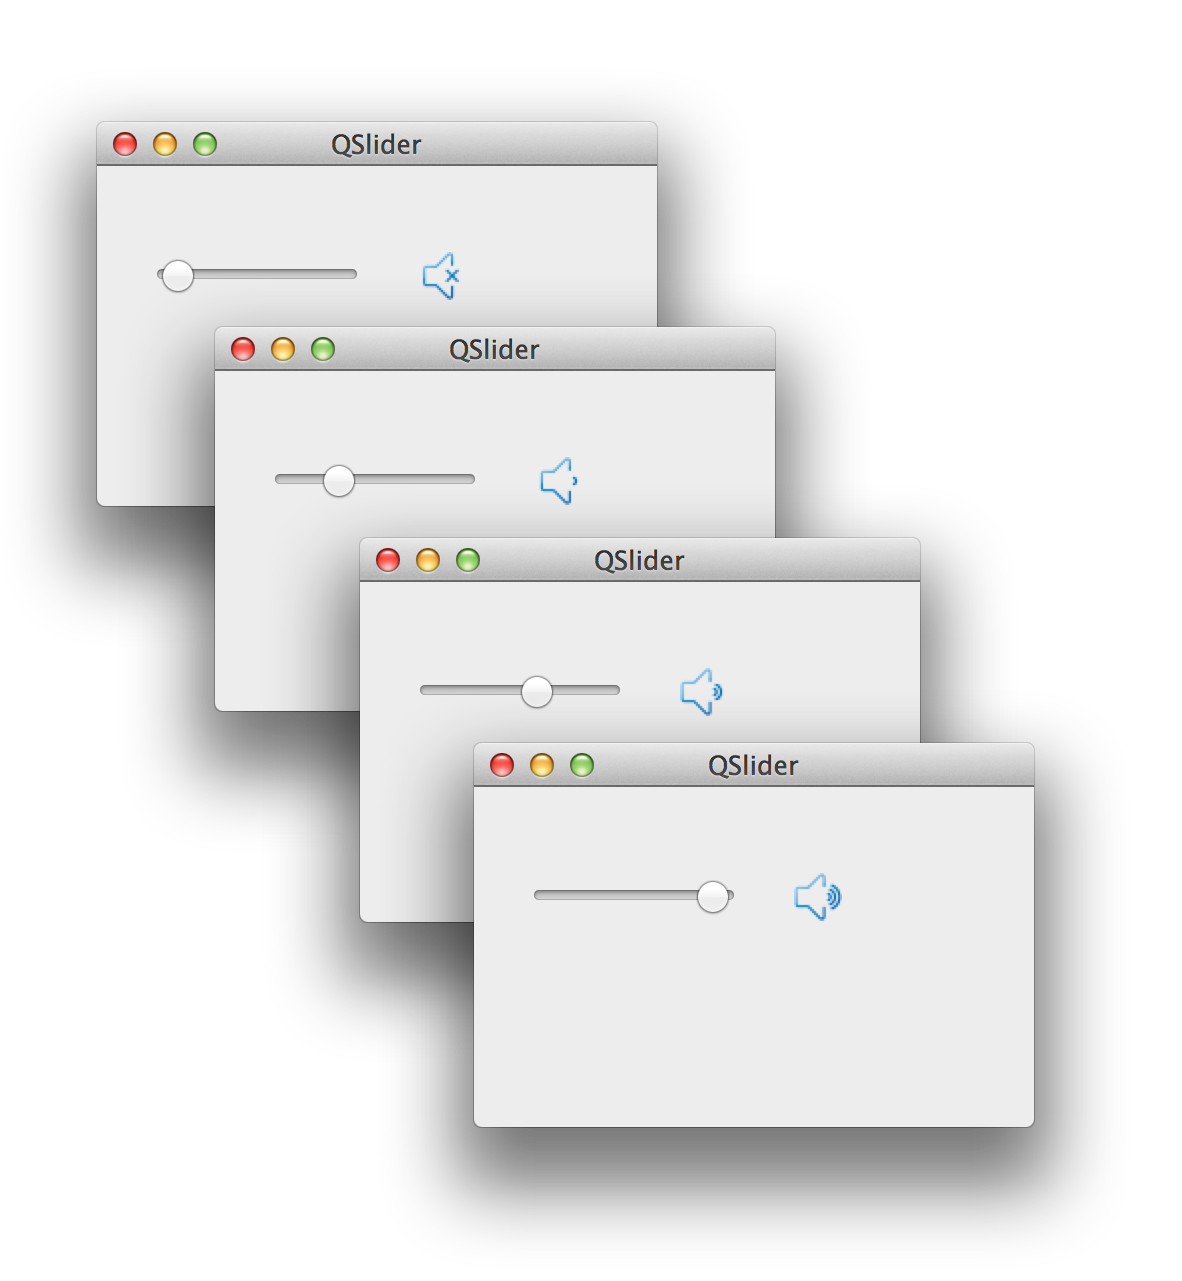
\includegraphics[scale=0.17]{pyqt14.png}
\end{center}
\end{frame}

\begin{frame}[fragile,shrink]
  \frametitle{QProgressBar}
\begin{minted}{python}
class Example(QtGui.QWidget):
    def initUI(self):
        self.pbar = QtGui.QProgressBar(self)
        self.pbar.setGeometry(30, 40, 200, 25)
        self.btn = QtGui.QPushButton('Start', self)
        self.btn.move(40, 80)
        self.btn.clicked.connect(self.doAction)
        self.timer = QtCore.QBasicTimer()
        self.step = 0
        ...
    def timerEvent(self, e):      
        if self.step >= 100:
            self.timer.stop()
            self.btn.setText('Finished')
            return
        self.step = self.step + 1
        self.pbar.setValue(self.step)

    def doAction(self):
        if self.timer.isActive():
            self.timer.stop()
            self.btn.setText('Start')
        else:
            self.timer.start(100, self)
            self.btn.setText('Stop')
\end{minted}
\end{frame}

\begin{frame}[fragile]
  \frametitle{QProgressBar $_2$}
\begin{center}
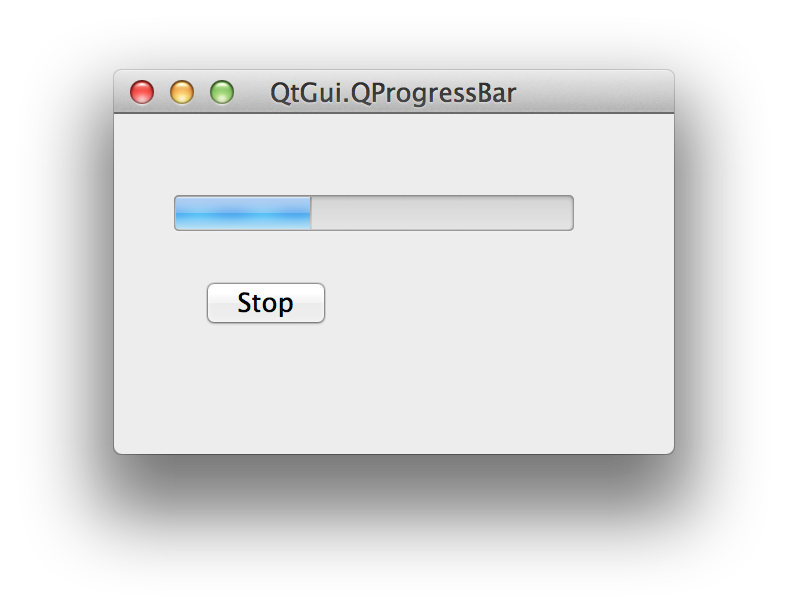
\includegraphics[scale=0.5]{pyqt15.png}
\end{center}
\end{frame}

\begin{frame}[fragile,shrink]
  \frametitle{QComboBox}
\begin{minted}{python}
class Example(QtGui.QWidget):
    def initUI(self):
        self.lbl = QtGui.QLabel("Ubuntu", self)
        combo = QtGui.QComboBox(self)
        combo.addItem("Ubuntu")
        combo.addItem("Mandriva")
        combo.addItem("Fedora")
        combo.addItem("Red Hat")
        combo.addItem("Gentoo")
        combo.activated[str].connect(self.onActivated)        
        ...
    def onActivated(self, text):
        self.lbl.setText(text)
        self.lbl.adjustSize()  
\end{minted}
\end{frame}

\begin{frame}[fragile]
  \frametitle{QComboBox $_2$}
\begin{center}
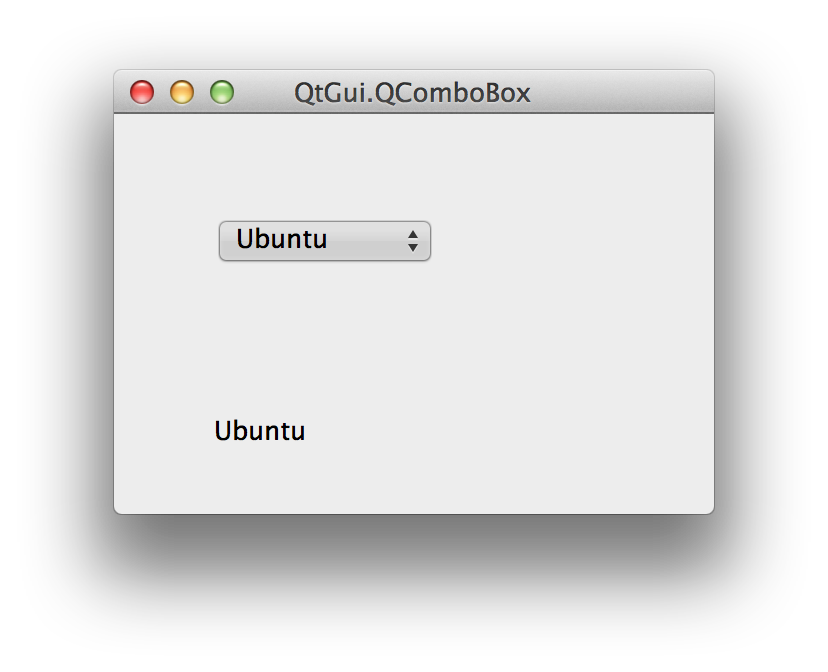
\includegraphics[scale=0.5]{pyqt16.png}
\end{center}
\end{frame}

\begin{frame}[fragile,shrink]
  \frametitle{Pravljenje sopstvene komponente}
\begin{minted}{python}
class Example(QtGui.QWidget):
    def initUI(self):
        self.text = u'\u041b\u0435...'

    def paintEvent(self, event):
        qp = QtGui.QPainter()
        qp.begin(self)
        self.drawText(event, qp)
        qp.end()
        
    def drawText(self, event, qp):
        qp.setPen(QtGui.QColor(168, 34, 3))
        qp.setFont(QtGui.QFont('Decorative', 10))
        qp.drawText(event.rect(), QtCore.Qt.AlignCenter, 
            self.text)        
\end{minted}
\end{frame}

\begin{frame}[fragile]
  \frametitle{Pravljenje sopstvene komponente $_2$}
\begin{center}
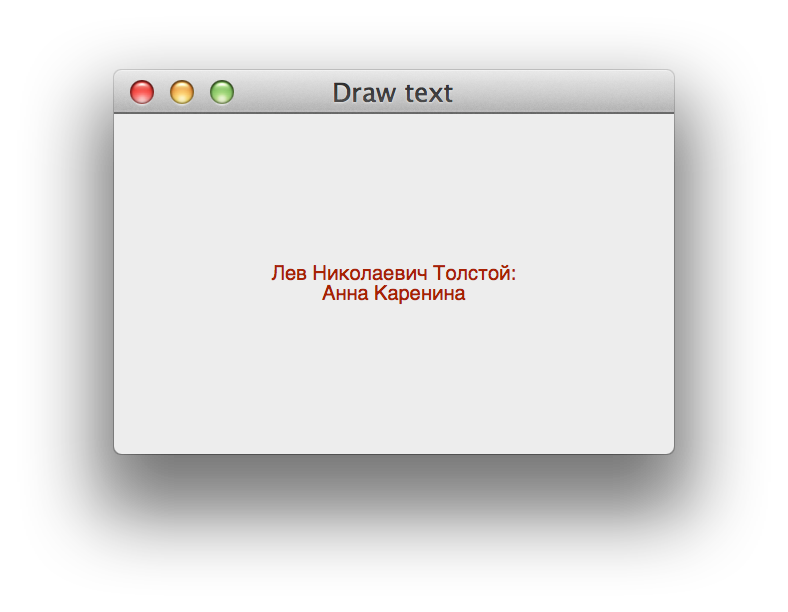
\includegraphics[scale=0.5]{pyqt17.png}
\end{center}
\end{frame}

\section[Tetris]{Tetris igra}

\begin{frame}[fragile]
  \frametitle{Primer: Tetris}
\begin{center}
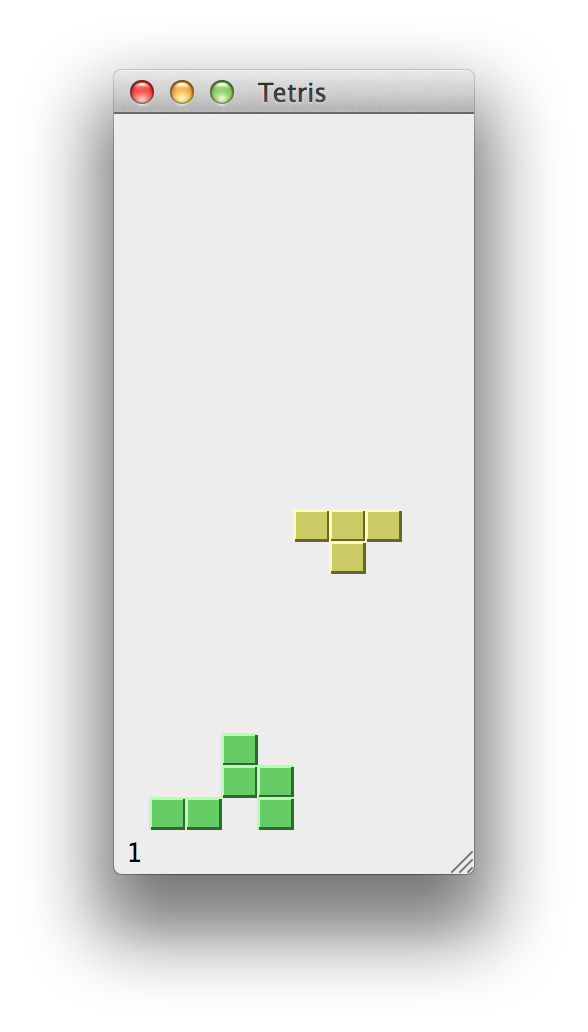
\includegraphics[scale=0.45]{pyqt18.png}
\end{center}
\end{frame}

\begin{frame}[fragile]
  \frametitle{Tetris: 4 klase}
  \begin{itemize}
    \item \texttt{Tetris}
    \begin{itemize}
      \item inicijalizuje igru
    \end{itemize}
    \item \texttt{Board}
    \begin{itemize}
      \item sadrži logiku igre
    \end{itemize}
    \item \texttt{Tetrominoe}
    \begin{itemize}
      \item sadrži imena svih delova
    \end{itemize}
    \item \texttt{Shape}
    \begin{itemize}
      \item implementira ponašanje jedne figure
    \end{itemize}
  \end{itemize}
\end{frame}

\end{document}